%************************************************
\section{Asymmetry of Drosophila ON and OFF motion detectors enhances real-world velocity estimation}
% \section{Leonhardt et al., 2016}
\label{sct:manuscript_leonhardt}
%************************************************

In this article, we studied the link between natural scene statistics and asymmetric tuning properties of ON and OFF pathways in the \textit{Drosophila} visual system. The paper was published in \textit{Nature Neuroscience} in May 2016 \citep{Leonhardt:2016ex}.

\paragraph{Summary}
To study motion vision, we commonly make use of simplified, easily parameterized stimuli like sine gratings or edges. Animals, however, solve the problem of detecting direction in natural environments which have varied and complex statistical structure. Here, we attempted to connect the two settings. We examined the transfer function between the velocity of translating natural images and the magnitude of the optomotor response performed by walking fruit flies. Interestingly, this yielded high correlation values which were not substantially affected by silencing T4 or T5 individually, suggesting that both pathways are well adapted to the task. When we examined the velocity tuning of the two pathways using polarity-specific edge stimuli, we found strong asymmetries: for OFF edges, both responses of tangential cells and walking behavior were tuned to higher velocities than for ON stimuli. We optimized the \textit{in silico} velocity estimation performance of an algorithmic motion detector for a large set of natural images and found ON-OFF asymmetries that closely resembled our empirical findings. When we scrambled the higher-order structure of the images, these asymmetries disappeared. Our findings suggest that ON and OFF pathways in fly motion vision are precisely tuned to the particular demands of natural scenes.

\paragraph{Authors} \textbf{Aljoscha Leonhardt}, Georg Ammer (co-first author), Matthias Meier, Etienne Serbe, Armin Bahl, and Alexander Borst.

\paragraph{Contributions}
\textbf{A.L.}, G.A.\ and A.\ Borst designed the study. \textbf{A.L.}\ performed behavioral experiments, associated data analysis and all modeling work. G.A., M.M.\ and E.S.\ performed electrophysiological experiments. G.A.\ performed calcium imaging. \textbf{A.L.}\ and G.A.\ analyzed physiological data. A.\ Bahl designed the behavioral apparatuses and performed behavioral experiments. \textbf{A.L.}\ wrote the manuscript with help from all of the authors.

\cleardoublepage

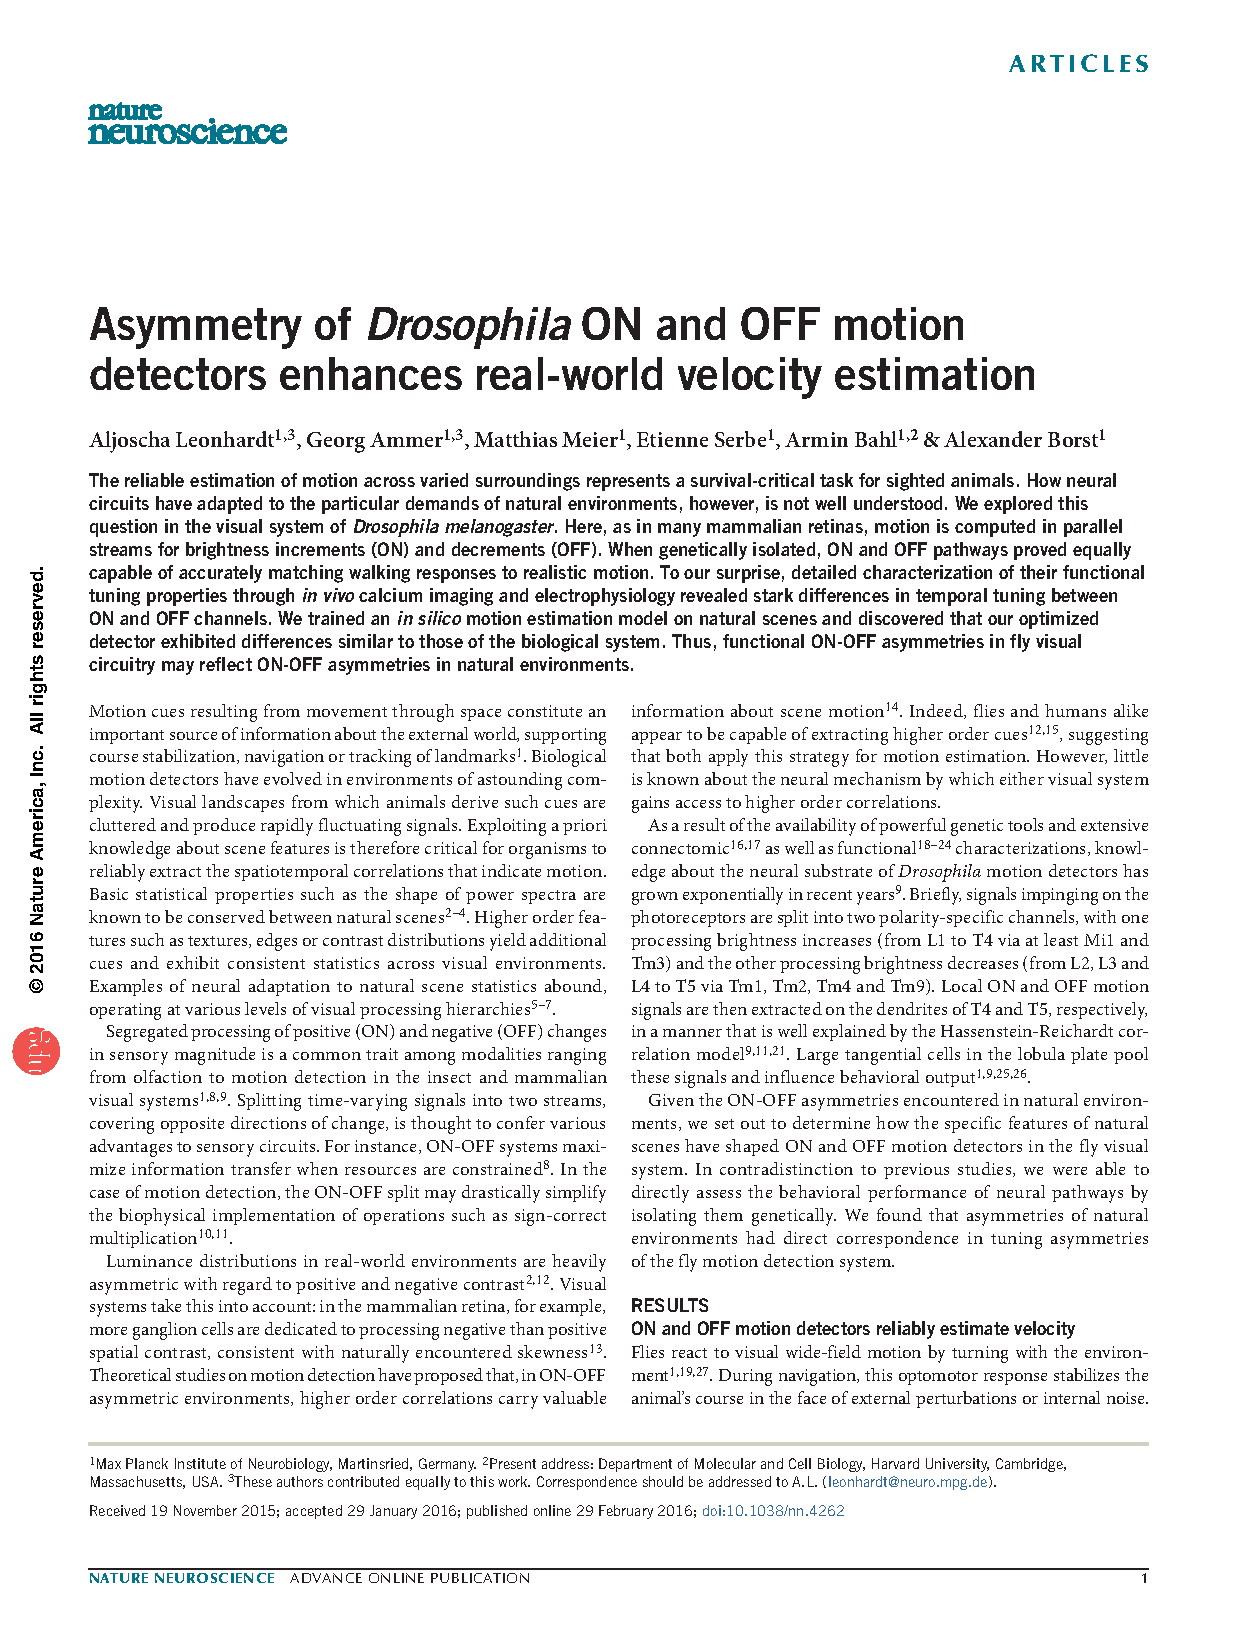
\includepdf[pages=-,scale=0.9,offset= 0 40,pagecommand={\thispagestyle{plain}}]{papers/leonhardt2016}
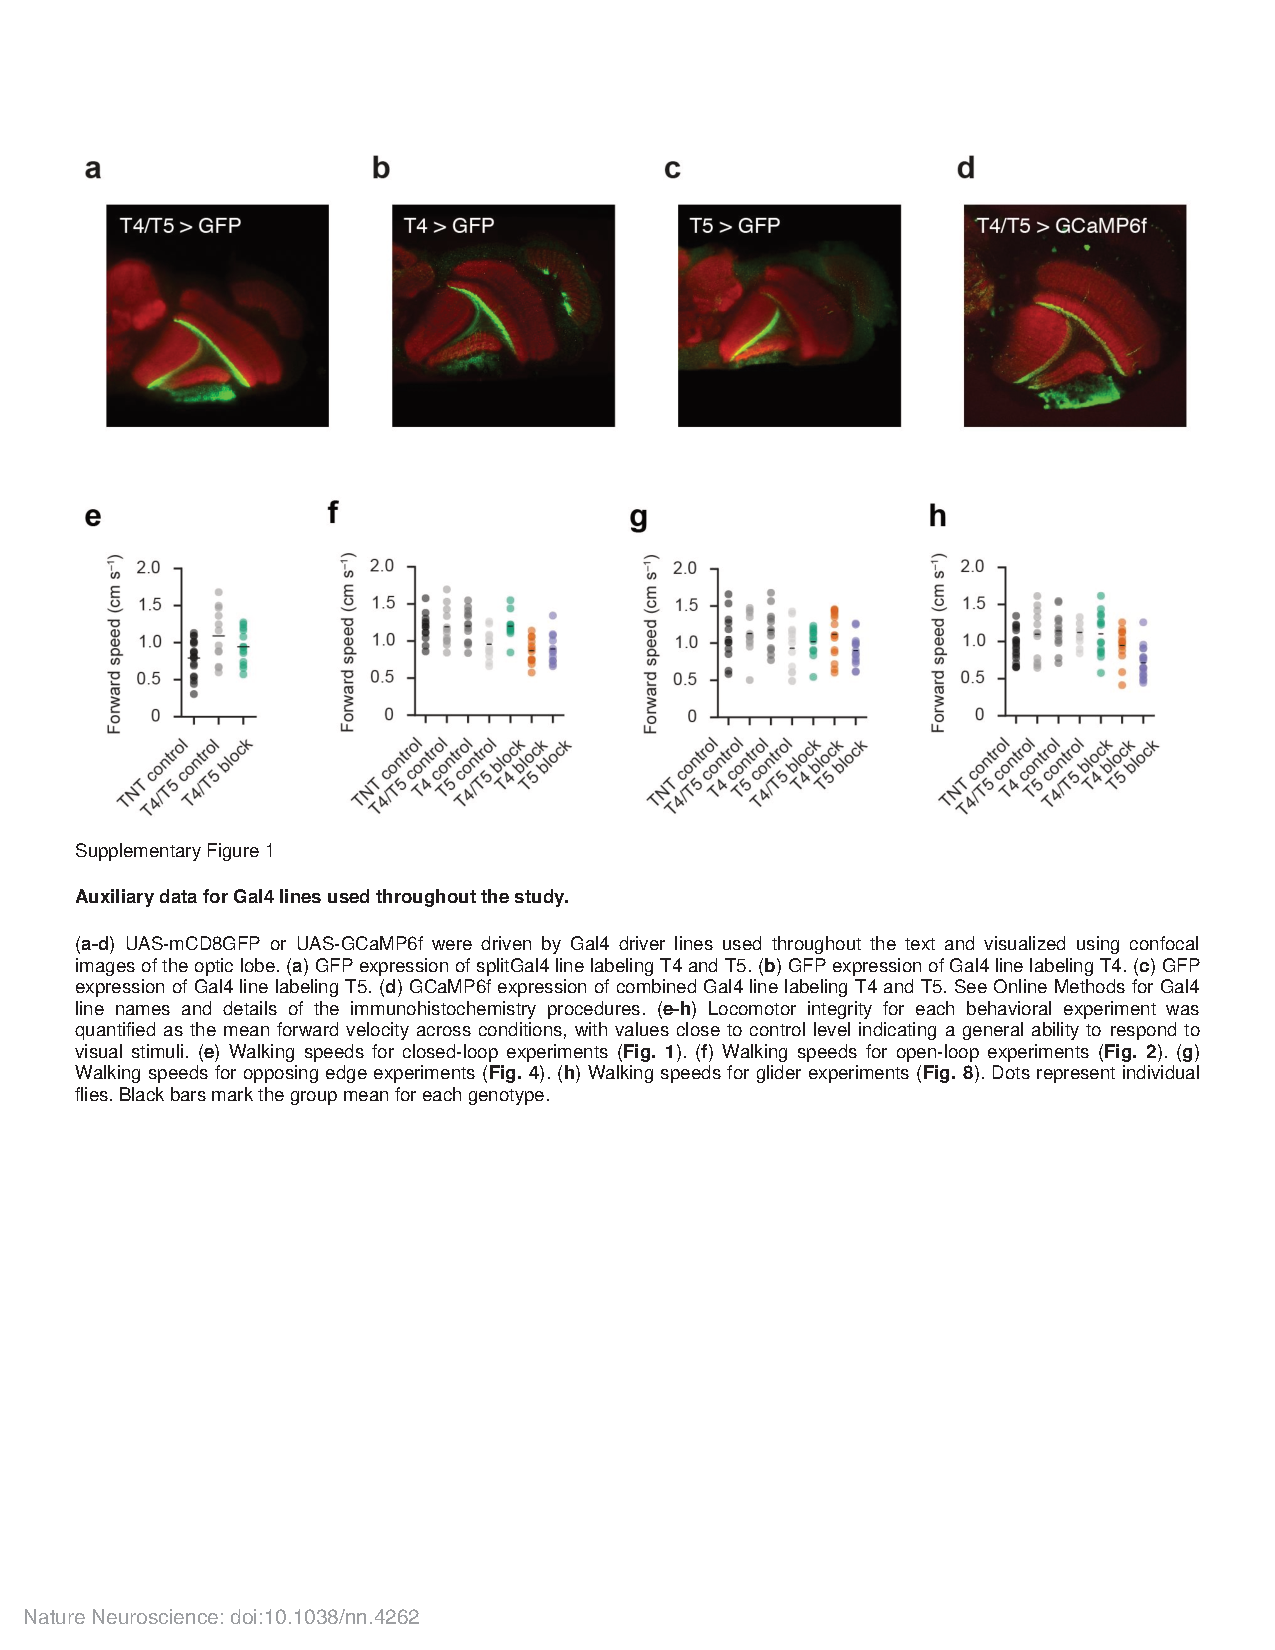
\includepdf[pages=-,scale=0.9,offset= 0 40,pagecommand={\thispagestyle{plain}}]{papers/leonhardt2016_supplement}